\documentclass[man,floatsintext,donotrepeattitle,a4paper]{apa6}

%Alles fürs Zitieren und die bib
\usepackage[utf8]{inputenc} 
\usepackage{csquotes}
\usepackage[style=apa,sortcites=true,sorting=nyt,backend=biber]{biblatex}
\DeclareLanguageMapping{german}{german-apa}
\addbibresource{bib2.bib}
\usepackage{textcomp}
\usepackage{hyperref}


%Tabelle
\usepackage{multirow}
\usepackage{tabularx}
\usepackage{booktabs}	
\newcolumntype{G}{>{\raggedright\arraybackslash}X}
\newcolumntype{L}[1]{>{\raggedright\arraybackslash}p{#1}}
\newcolumntype{C}[1]{>{\centering\arraybackslash}p{#1}}
\usepackage{color}															 % 
\usepackage{colortbl}	
\definecolor{hellgrau}{rgb}{0.95,0.95,0.95}

%Kram
\usepackage[ngerman]{babel}
\usepackage[T1]{fontenc}
\usepackage{amsmath}
\usepackage{amsfonts}
\usepackage{amssymb}
\usepackage{todonotes}
\usepackage{lipsum}


\usepackage{blindtext}
\makeatletter
\def\flushboth{%
      \let\\\@normalcr
        \@rightskip\z@skip \rightskip\@rightskip
          \leftskip\z@skip
            \parindent 1.5em\relax}
\makeatother

%Titel
\author{Katharina Drawert, Moritz Mager}
\leftheader{Drawert, Mager}
\affiliation{Leuphana Universität Lüneburg}
\title{Erfolg von Massive Open Online Courses - messbar?}
\shorttitle{MOOC Analyse}

%Abstract
\abstract{
\flushboth
\blindtext

1. Function: An abstract summarizes, in one paragraph (usually), the major aspects of the entire paper in the following prescribed sequence:

    the question(s) you investigated (or purpose), (from Introduction)
        state the purpose very clearly in the first or second sentence. 
    the experimental design and methods used, (from Methods)
        clearly express the basic design of the study.
        Name or briefly describe the basic methodology used without going into excessive detail-be sure to indicate the key techniques used. 
    the major findings including key quantitative results, or trends (from Results)
        report those results which answer the questions you were asking
        identify trends, relative change or differences, etc. 
    a brief summary of your interpetations and conclusions. (from Discussion)
        clearly state the implications of the answers your results gave you. 
}

\keywords{MOOC, SEM, IS Success}

%Los geht's
\begin{document}
\maketitle
\flushboth
\section{Einleitung}
\label{sec:einleitung}

Die Vermittlung von Wissen in einem universitären Kontext beschränkte sich bis zu der flächendeckenden Verbreitung des Internets in Privathaushalten auf die lokale Anwesenheit in Vorlesungen, Seminaren oder Kursen. Die ersten e-Learning Angebote konnten jedoch erstmals auch unabhängig von örtlicher Gebundenheit genutzt werden. Massive Open Online Courses (MOOC) hingegen ermöglichen die Verlagerung ganzer Veranstaltungen ins Internet und unterscheiden sich somit zu klassischen e-Learning Angeboten, die meist nur zu einem bestimmten Themengebiet medial aufbereitete Erklärungen bieten.
\newline
In der wissenschaftlichen Fachliteratur sind bereits einige Untersuchungen über den Erfolg von e-Learnings durchgeführt worden. Im Bereich von MOOCs hingegen sind eher wenige Studien vorhanden. Gerade die Frage, wodurch der Erfolg der einzelnen Teilnehmer eines MOOCs entscheidend beeinflusst wird, wurde bisher unzureichend untersucht. Um dieser Fragestellung nachzugehen, sind deutliche Parallelen zu e-Learnings festzustellen. Es bietet sich daher an, Teile von existierenden Forschungsmodellen auf diesen Bereich anzuwenden. Die Datenbasis ergibt sich aus beantworteten Fragebögen, die zu unterschiedlichen Zeiten an Teilnehmer eines MOOCs der Leuphana Digital School versendet wurden. 
%Zitattest
\section{Grundlagen}
\label{sec:grundlagen}

\cite{king2006meta} sagten:" \blindtext" \parencite{behrenbruch2013understanding}
%Grafiktest
\section{Modell}
\label{sec:modell}
Das IS Success Modell wurde als Basis genommen, um die die Einflussfaktoren eines MOOCs zu analysieren. Als relevante Konstrukte wurde dabei Systemqualität, Servicequalität, Nutzerzufriedenheit und Net Benefits identifiziert.  

In der Vergangenheit konnte bereits in diversen Studien zu IS Success-Modellen - unter anderen im e-Learning-Bereich - die Bedeutung der Systemqualität auf die Nutzerzufriedenheit bestätigt werden (Alsabawy et al., 2013; Motaghian et al., 2013; Saba, 2013; Tajuddin et al., 2013; Hassanzadeh et al., 2012; Kim et al., 2012; Islam, 2012; Wang and Chiu, 2011; Rai et al., 2009; Wu et al., 2008), daher gilt auch hier die Hypothese: \medskip

\textbf{H1:} \textit{Die Systemqualität hat einen positiven Einfluss auf die Nutzerzufriedenheit.} \medskip

Die Servicequalität im IS Success-Modell wurde von manchen Autoren in der Literatur kritisch betrachtet \todo{Quellen, kritisch gegenüber Servicequalität)}. Dabei wurde unter Servicequalität vorwiegend der Support verstanden, den Nutzer vom IS erhalten konnten, wie z.B. Training (\parencite{petter2009meta}) oder Helpdesk. Im Rahmen eines MOOCs wird unter Servicequalität allerdings vorwiegend die (Online-)Betreuung durch Mentoren, Lehrende und Mitarbeiter des MOOC-Anbieters verstanden. Aus diesem Grund wird der Servicequalität ein maßgeblicher Einfluss auf die Nutzerzufriedenheit eingeräumt: \medskip

\textbf{H2:} \textit{Die Servicequalität hat einen positiven Einfluss auf die Nutzerzufriedenheit.}\medskip

Der Term "`Net Benefit"' wird von dem neuformulierten IS Success Modell übernommen. Er besagt, dass es sich um ein positives Ergebnis (Benefit) handelt, was allerdings auch negative Einflüsse enthalten kann (Net) \parencite[vgl.][S.2974]{delone2002information}. Der Erfolg eines MOOCs kann aus verschiedenen Perspektiven gemessen werden, z.B. aus Sicht des Teilnehmers, des MOOC Anbieters, der Lehrenden, des Systemanbieters etc. Jede Perspektive hätte eine andere Definition von Net Benefit zur Folge. In erster Linie sollte der Erfolg eines MOOCs an den Teilnehmern sichtbar sein, daher wird in dieser Studie der Erfolg des MOOCs aus der individuellen Sicht des Teilnehmers gemessen. Eine hohe Nutzerzufriedenheit wurde in vergangenen Studien bereits als Einflussgröße für den Net Benefit ermittelt (\todo{Quellen Studien} und stimmt mit dem IS Success Modell überein. Die empirische Datenerhebung fand auf Basis eines MOOCs der Leuphana Digital School (LDS) statt (siehe \nameref{sec:emp_daten}). Die LDS definiert MOOC als "`Mentored Open Online Course"' und weist der Servicequalität damit eine besondere Bedeutung zu. Daher wird in diesem Rahmen - im Gegensatz zum herkömmlichen IS Success Modell - auch von einem positiven Einfluss der Servicequalität auf den Net Benefit ausgegangen. Die weiteren Hypothesen lauten entsprechend: \medskip


\textbf{H3:} \textit{Die Servicequalität hat einen positiven Einfluss auf den Net Benefit.} 


\textbf{H4:} \textit{Die Nutzerzufriedenheit hat einen positiven Einfluss auf den Net Benefit.} \medskip


Die Konstrukte Informationsqualität und Nutzung, bzw. beabsichtigte Nutzung werden - unter anderem aus Vereinfachungsgründen - in dem hier behandelten Modell nicht berücksichtigt. Das Wegfallen des Konstruktes Nutzung folgt dabei der Argumentation von \cite{seddon1997respecification}, der angibt, dass Nutzung keine Erfolgsvariable in einem Kausalmodell darstellt. 

Daher 
Das im Rahmen dieses Papers verwendete IS Success Modell beinhaltet allerdings nur 4 Konstrukte, da erstens die Anzahl der Fragen streng reglementiert war und darüber hinaus auch nur eine geringe Response Rate erwartet wurde. Somit ist es mit dem kleinen sample besser möglich, qualitativ gute Aussagen zu treffen. Die Konstrukte sind in Tabelle \ref{tab:Forschungsmodell} genau definiert.

\todo{Warum andere Konstrukte ausgeschlossen?? Inhaltliche Erklärung}

Table 2
Definitions of dimensions.

% Tabellenformat 2
\begin{table}[ht] 
\footnotesize
\caption{Definition der Dimensionen}
\label{tab:Dimensionen} 
\begin{tabular}{@{}lp{9cm}l@{}} \toprule

\textbf{Konstrukt} & \textbf{Definiton} & \textbf{Quelle} \\ \midrule


Servicequalität 	& Qualitätsfaktor für die erwarteten Support,den die Nutzer in Anspruch nehmen können & \parbox[t]{4cm}{\cite{petter2008measuring}}\\ 

Systemqualität 		& Die erwarteten Eigenschaften und Funktionen von dem System & \parbox[t]{4cm}{\cite{petter2008measuring}}\\ 

Nutzerzufriedenheit & Das Ausmaß darüber, in wie weit die Bedürfnisse, Ziele und Wünsche während des MOOC erfüllt werden & \parbox[t]{4cm}{\cite{sanchez2009moderating}}\\ 

Net Benefit 		& Drückt aus, inwieweit Informationssysteme zum Erfolg einzelner Personen, Gruppen und Organisation beitragen können  & \parbox[t]{4cm}{\cite{conf/gi/GemlikNSB10} \cite{Petter:0aa} }\\ \addlinespace 
  \bottomrule

\end{tabular}	
\end{table}



\section{Empirische Datenbasis}
\label{sec:emp_daten}

Forschungsmethode

Für die Untersuchung der Hypothesen und der Darstellung der Ergebnisse wurde während eines Massive Open Online Course zu drei Zeitpunkten ein Fragebogen an die Teilnehmer versendet. Schon bei der Konzeption des Fragebogens musste das Modell für die anschließende Auswertung der Daten feststehen, da die Fragen entsprechend gestellt werden mussten. In diesem Kontext wird dazu häufig ein Modell von DeLone und McLean angewandt, welches international unter dem Namen "`IS Success Model"' bekannt ist. Die Erfolgsmessung von Informationssystemen verfolgt dabei einem bestimmten Muster und ermöglicht somit Vergleiche mit anderen Erhebungen. Seit der ersten Entwicklung im Jahr 1992 wurde das Modell intensiv diskutiert und dabei empirisch auf die Qualität hin überprüft. Grundlegend stellten DeLone und McLean fest, dass sich fast alle Erfolgsmessungen in nur sechs Kategorien einordnen lassen, die untereinander als abhängige Variablen dargestellt werden können. Im Laufe der wissenschaftlichen Weiterentwicklung wird in der Literatur das aktuelle Modell wie in Abbildung grafisch dargestellt. (vlg. \cite{delone2002information})

\begin{figure}[h]
\centering
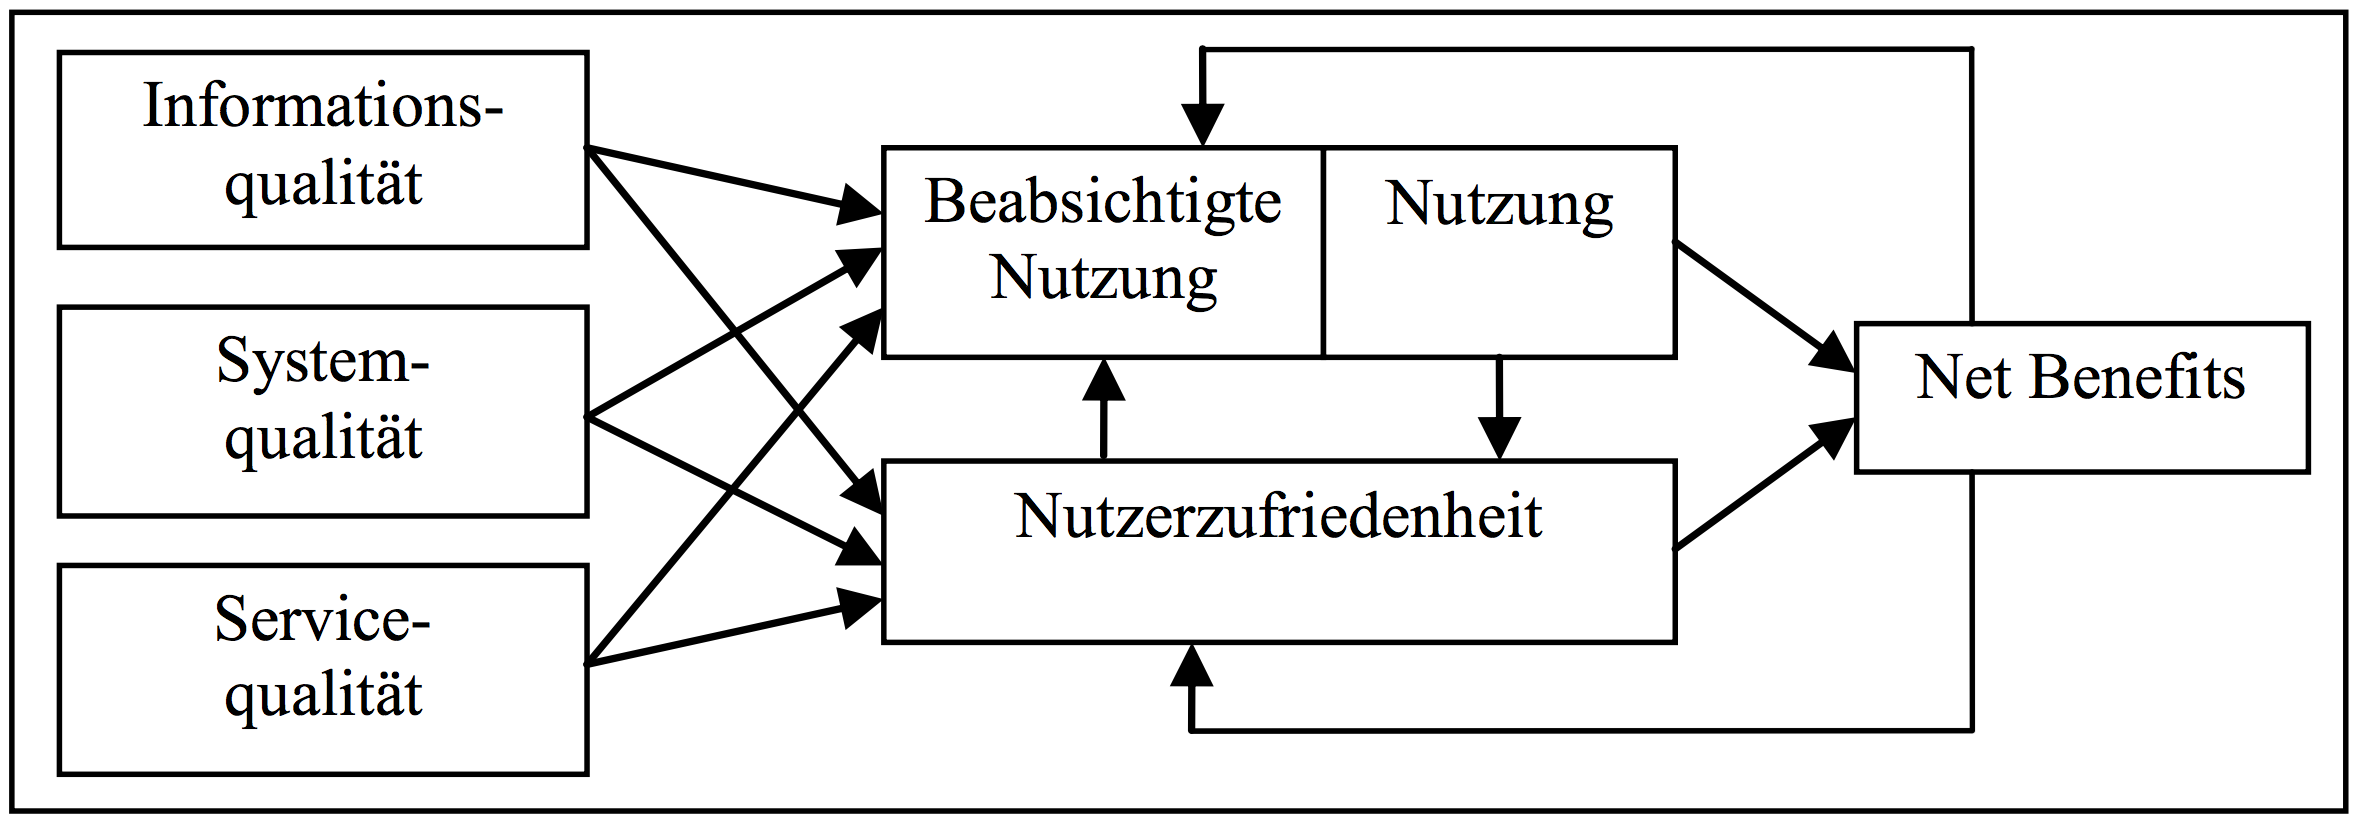
\includegraphics[width=1\textwidth]{Grafiken/issuccess.png}
\caption{IS Success Modell}
\label{IS Success Model}
\end{figure}



\label{tab:Forschungsmodell} 

Das im Rahmen dieses Papers verwendete IS Success Modell beinhaltet allerdings nur 4 Konstrukte, da erstens die Anzahl der Fragen streng reglementiert war und darüber hinaus auch nur eine geringe Response Rate erwartet wurde. Somit ist es mit dem kleinen sample besser möglich, qualitativ gute Aussagen zu treffen. Die Konstrukte sind in Tabelle \ref{tab:Forschungsmodell} genau definiert. Die vorliegenden Daten entstammen aus Befragungen der Teilnehmer des MOOCs  \textit{Psychology of Negotiations - Reaching Sustainable Agreements in Negotiations on Commons}  der Leuphana Digital School. Der Kurs fand von Mai bis August 2014 statt und war offen für Teilnehmer aus der ganzen Welt. Die Teilnehmerzahl wurde auf 1000 begrenzt um die Qualität der Beratung und Führung durch Mentoren und Lehrende zu gewährleisten. Der Kurs selbst war gebührenfrei, jedoch konnten die Teilnehmer mit einem erfolgreichen Abschluss des Kurses ein Zertifikat der Universität erhalten, welches gegen eine Gebühr von 20 \texteuro " " ausgestellt wurde. Für die Anrechnung in einem Hochschulstudium können damit maximal 5 Credit Points (ECTS) angerechnet werden. Aufgrund der internationalen Ausrichtung des Kurses wurden die Fragen in Englisch gestellt, wobei eine Seven-point Likert Skala verwendet wurde. Die Antwortmöglichkeiten reichten von "`Strongly disagree (1)"' bis "`Strongly Agree (7)"'. Wie eingehend schon erwähnt, fand die Erhebung der Daten zu drei unterschiedlichen Zeitpunkten statt: zu Beginn des Kurses (T1), während des Kurses (T2) und zum Ende des Kurses (T3). Die Beantwortung der Umfrage unterlag einer freiwilligen Basis. Die im Forschungsmodell beschriebenen Items sind in den Fragebögen T2 und T3 enthalten. \todo{ITEM Enriched knowledge genau benennen}.
Für die Erstellung des Modells konnten jedoch nur Daten aus T2 und T3 verwendet werden, da die Teilnehmer zu Beginn des Kurses keine Angaben über ihren persönlichen Erfolg machen konnten (Frageitem: Enriched Knowledge fehlt in T1).  
 
% Tabellenformat 2

\begin{table}[ht] 
\footnotesize
\caption{Forschungsmodell}
\label{tab:Forschungsmodell} 
\begin{tabular}{@{}lp{10cm}r@{}} \toprule

\textbf{Konstrukt} & \textbf{Item} & \textbf{Factorloadings} \\ \midrule

Servicequalität & The Leuphana Digital School provides a proper level of online assistance and explanation & 0,794\\ 
& The teaching staff is highly availability for consultation & 0,913 \\
& The teaching staff provides satisfactory support to users using Leuphana Digital School & 0,887 \\ 
Systemqualität & Leuphana Digital School’s technical system has attractive features to appeal to the users. & 0,895\\ 
& Leuphana Digital School’s technical system is easy to use. & 0,865 \\
& Leuphana Digital School’s technical system provides a personalized information presentation. & 0,808 \\ 
Nutzerzufriedenheit & Most of the users bring a positive attitude or evaluation towards Leuphana Digital School. & 0,763\\ 
& Leuphana Digital School’s technical system is easy to use. & 0,865 \\ 
Net Benefit & Leuphana Digital School helps you think through problems.  & 0,927\\ 
& All in all, my knowledge has been enriched as a result of the course & 0,768 \\ \addlinespace 
  \bottomrule

\end{tabular}	
\end{table}


% Tabellenformat 2

\begin{table}[ht] 
\caption{Forschungsmodell2}
\label{tab:Forschungsmodell} 
\begin{tabular}{@{}lp{12cm}r@{}} \toprule

\textbf{Konstrukt} & \textbf{Item} \\ \midrule

Servicequalität & The Leuphana Digital School provides a proper level of online assistance and explanation \\ \addlinespace
& The teaching staff is highly availability for consultation\\\addlinespace
& \parbox[t]{12cm}{The teaching staff provides satisfactory support to users using Leuphana Digital School} \\ \addlinespace
Systemqualität & \parbox[t]{12cm}{Leuphana Digital School’s technical system has attractive features to appeal to the users.}\\ \addlinespace
& Leuphana Digital School’s technical system is easy to use. \\\addlinespace
& \parbox[t]{12cm}{Leuphana Digital School’s technical system provides a personalized information presentation.} \\ \addlinespace
Nutzerzufriedenheit & \parbox[t]{12cm}{Most of the users bring a positive attitude or evaluation towards Leuphana Digital School.} \\ \addlinespace
& Leuphana Digital School’s technical system is easy to use.  \\ \addlinespace 
Persönlicher Nutzen & \parbox[t]{12cm}{Leuphana Digital School helps you think through problems.} \\ \addlinespace 
& \parbox[t]{12cm}{All in all, my knowledge has been enriched as a result of the course (nur in Fragebogen 2 und 3)} \\ \addlinespace 
  \bottomrule

\end{tabular}	
\end{table}

Teilnehmer
   
Die Fragebögen wurden an alle Teilnehmer verschickt. Da die Anzahl der Kursteilnehmer, die den Fragebogen erhalten haben unbekannt ist, kann die Returnquote nicht angegeben werden. Gemessen an den Antworten, ist diese jedoch eher gering - vor allem in T2 und T3. Bei Ersterem lagen 32 Antworten vor, wovon nach Bereinigung von ungültigen oder unvollständigen Antworten 29 verwertbare waren. Die Bereinigung ungültiger und unvollständiger Antworten reduzierte die nutzbaren Antworten in T3 von 48 auf 36. Insgesamt liegen damit 65 Datensätze für die Modellüberprüfung vor, was einen relativ kleinen Stichprobenumfang darstellt. \cite[S. 5]{jakobowicz2006understanding} gaben an, dass für ein komplexes Modell ein Stichprobenumfang von mindestens 200 empfehlenswert ist, da ein geringer Stichprobenumfang zu Verzerrungen bei der Parameterschätzung und einem großem Standardfehler führen. Das in dieser Arbeit überprüfte Modell ist mit zwei unabhängig latenten (Systemqualität und Servicequalität) und zwei abhängig latenten Variablen (Nutzerzufriedenheit und Persönlicher Nutzen) verhältnismäßig einfach, daher kann auch ein kleiner Stichprobenumfang ausreichend Erkenntnisse liefern, gleichzeitig sollte bei der Interpretation der Ergebnisse jedoch der Stichprobenumfang berücksichtigt werden. 
Die Demographischen Daten der Fragebögen T2 und T3 lassen sich aus Tabelle\,\ref{tab:Demographische Daten} entnehmen. 
 

\begin{table}[ht] 
\footnotesize
\caption{Demographische Daten}
\label{tab:Demographische Daten} 
\begin{tabular}{@{}lp{5cm}r@{}} \toprule

 & \textbf{Anzahl}&\textbf{in Prozent} \\ \midrule

\textit{Geschlecht}		& 				& \\ 
weiblich 				&  40 			& 62 \\
männlich				&  25			& 38 \\ 
Total					&  65			& 100 \\
\textit{Alter}			& 				&   \\
21-30 Jahre				&  35			& 54 \\
31-40 Jahre				&  10			& 15	  \\
> 41 Jahre				&  20 			& 31 \\
Total 					&  65			& 100 \\
\textit{Herkunft}		&				&   \\
Deutschland				& 27 			& 42  \\
Europa (excl. Deutschland) &18			& 28  \\
Afrika 					& 6				& 9   \\
Asien 					& 6				& 9   \\
Nordamerika				& 4				& 6   \\
Südamerika				& 4				& 6	 \\
Total					& 65				& 100  \\ 
  \bottomrule

\end{tabular}	
\end{table}


Data Analysis Technique
Instrument validation
We followed the procedures outlined by Gefen and Straub (2005) to test discriminant and convergent validity. Discriminant validity refers to whether the items measure the construct in question or other (related) constructs (Gefen and Straub, 2005). We verified discriminant validity using correlation matrix and factor analysis. Table 4 shows the correlation matrix with the square root of average variance extracted (AVE) values presented diagonally. The square root of the AVE value for the variables is consistently greater than the off-diagonal correlation values, suggesting satisfactory discriminant validity between the variables (Fornell and Larcker, 1981)

Zur Analyse im Rahmen dieser Arbeit wurde auf Strukturgleichungsmodellierung zurückgegriffen, 
For this paper, structural equation modeling (SEM) using partial least squares (PLS) was used to evaluate the research model and hypotheses.




%Tabellentest
\section{Ergebnisse}
\label{sec:ergebnisse}
\nocite{lohmoller2013latent}
Zur Evaluierung des Forschungsmodells und der Hypothesen wurde die Partial-Least-Square(PLS)-Methode verwendet. Dabei werden "`die Modellparameter so geschätzt, dass der Anteil der erklärten Varianz der abhängigen Variable und der Indikatoren eines reflektiv gemessenen Konstrukts maximiert wird"' \parencite[S.16]{nitzl2010anwenderorientierte}. Ein besonderer Vorteil der PLS-Methode ist ihre Anwendungsmöglichkeit auch bei verhältnismäßig kleiner Stichprobengröße. Zur Kalkulation einer minimalen Stichprobengröße kommt häufig eine Faustregel zur Anwendung, nach der die Stichprobengröße mindestens das zehnfache des Konstruktes mit der größten Anzahl zu schätzender Parameter sein sollte \parencite[vgl.][S.394]{islam2013investigating}. Dieses Kriterium wird in dieser Studie erfüllt. Zur Analyse wurde die Softwareapplikation SmartPLS verwendet. 

Für die Modellbeurteilung wird zunächst das reflektive Messmodell (äußeres Messmodell) einer Güteprüfung unterzogen. Die Konvergenzvalidität wird anhand der Kriterien Indikatorreliabilität, Konstruktreliabilität und duchschnittlich erfassten Varianz (DEV) kritisch betrachtet, während die Validität mithilfe der Diskriminanzvalidität überprüft wird.

Die Indikatorreliabiltät testet, ob sich ein Indikator für die Messung einer latenten Variable eignet. Eine Faktorladung $\lambda$ > 0,7 gilt als signifikant \parencite[vgl.][S.24]{nitzl2010anwenderorientierte}. Der Wert wird von allen Indikatoren erreicht (siehe Tabelle \ref{tab:Forschungsmodell}). 

Die Konstruktreliabilität $\rho$ untersucht unter Einsatz der internen Konsistenz (Composite reliability (CR)) "`wie gut die Indikatoren eine latente Variable wiedergeben"' \parencite[S.25]{nitzl2010anwenderorientierte}. Ein Wert von $\rho$ $\geq$ 0,6 gilt als aktzeptabel \parencite[vgl.][S.212]{ringle2007beurteilung}. Das Messmodell weist $\rho$ > 0,8 auf und liegen damit über den Schwellenwert.  

Die durchschnittliche erfasste Varianz (DEV) "`setzt den Anteil der erklärten Varianz in Relation zum Messfehler einer latenten Variable"'  \parencite[S.25]{nitzl2010anwenderorientierte}. Ein Wert von DEV $\geq$ 0,5 stellt einen ausreichend hohen Wert dar. Die DEV liegt in dieser Studie mit DEV > 0,7 ebenfalls über dem genannten Schwellenwert und ist somit akzeptabel. Die entsprechenden Werte für die Konstruktreliabilität und die DEV können Tabelle \ref{tab:Übersicht Gütekriterien} entnommen werden.

Die Diskriminanzvalidilität hingegen "`gibt an, in welchem Ausmaß sich die Indikatoren eines Konstrukts von denen eines anderen Konstrukts unterscheiden"' \parencite[S.26]{nitzl2010anwenderorientierte}. Zur Überprüfung der Diskriminanzvalididtät kann das Fornell-Larcker-Kriterium und die Cross Loadings herangezogen werden. 
Bei ersterem wird die Wurzel der DEV einer latenten Variable verglichen mit jeder Korrelation dieser latenten Variable mit einer anderen latenten Variablen und sollte stets größer sein \parencite[vgl.][S.26]{nitzl2010anwenderorientierte}. Das Fornell-Larcker-Kriterium wird in dieser Studie erfüllt (siehe Tabelle \ref{tab:Fornell-Larcker-Kriterium}). Die Cross Loadings können Tabelle \ref{tab:Cross-Loadings} entnommen werden. Ein Indikator sollte dabei die stärkste Beziehung mit dem ihm zugeordneten Konstrukt aufweisen \parencite[vgl.][S.26]{nitzl2010anwenderorientierte}, was ebenfalls erfüllt ist.   \nocite{fornell1981evaluating}

Das Messmodell erfüllt damit alle Gütekriterien. Zur Beurteilung des Strukturmodells (inneres Messmodell) werden das Bestimmtheitsmaß R$^2$, die Pfadkoeeffizienten, die Effektstärke f$^2$ und die Prognoserelevanz Q$^2$ herangezogen.  

Die Werte für das Bestimmtheitsmaß R$^2$ sind in Tabelle \ref{tab:Übersicht Gütekriterien} enthalten. Das Bestimmtheitsmaß "`gibt den Anteil der erklärten Varianz im Verhältnis zur Gesamtvarianz an."' \parencite[S.32]{nitzl2010anwenderorientierte} Eine Einteilung relevanterer Schwellenwerte wurde von \cite[S.323]{chin1998partial} in einer Studie ermittelt. Die Werte für R$^2$ von 0,67, 0,33 und 0,19 wurden in "`substanziell"', "`mittelgut"' und "`schwach"' eingeteilt. In dieser Studie sind die R$^2$ dementsprechend als "`mittelgut"' (Nutzerzufriedenheit: 0,387 / persönlicher Erfolg: 0,369) einzustufen.

Als Schwellenwerte für die Effektstärke f$^2$ wurden von \cite[S.316f.]{chin1998partial} 0,02, 0,15 bzw. 0,35 ermittelt. Diese sagen aus, ob eine unabhängige latente Variable einen geringen, mittleren bzw. großen Einfluss auf eine abhängige latente Variable hat. Demnach weist Nutzerzufriedenheit auf den persönlichen Lernerfolg (f$^2$=0,306) einen mittleren Einfluss und Systemqualität auf Nutzerzufriedenheit (f$^2$=0,519) einen großen Einfluss aus. 

Die Pfadkoeeffizienten $\gamma$ geben die Stärke der Kausalbeziehung zwischen den latenten Variablen an. Sie können Werte zwischen -1 und 1 annehmen. Ein Wert Nahe 0 gilt als schwach. Als signifikant wird ein Wert kleiner -0,2 oder größer 0,2 angesehen \parencite[vgl.][S.11]{chin1998commentary}. In dieser Studie haben dementsprechend die Nutzerzufriedenheit auf den persönlichen Erfolg ($\gamma$ = 0,557; p < 0,001) und die Servicequalität auf die Nutzerzufriedenheit ($\gamma$ = 0,591; p < 0,001) einen signifikant positiven Einfluss. (siehe Abbildung...) Die mithilfe der Bootstrapping-Methode ermittelten T-Werte bestätigen die Signifikanz der beiden Pfadkoeffizienten. Die restlichen Hypothesen können hingegen nicht bestätigt werden. 

Das Geisser-Stone-Kriterium sieht eine ausreichende Prognoserelevanz wenn Q$^2$ > 0, was in dieser Studie erfüllt wurde (siehe Tabelle \ref{tab:Übersicht Gütekriterien}) 

Die Prognoserelevanz Q$^2$ wird nach dem Geisser-Stone-Kriterium überprüft, wonach man bei Q$^2$ > 0 von einer ausreichenden Prognoserelevanz spricht. Die Berechnung erfolgt mithilfe der Blindfolding-Methode in SmartPLS, die Ergebnisse lassen sich Tabelle \ref{tab:Übersicht Gütekriterien} entnehmen
 





\begin{table}[h] 
\footnotesize
\caption{Übersicht Gütekriterien}
\label{tab:Übersicht Gütekriterien} 
\begin{tabular}{@{}llllll@{}} \toprule

\textbf{Faktor} & \textbf{DVE} & \textbf{CR} & \textbf{R$^2$} & \textbf{Q$^2$} \\ \midrule

 Net Benefit 		& 0,725 		& 0,839 & 0,369 & 0,219 		 \\
 
 Servicequalität 	& 0,750 		& 0,900 & 		& 			 \\

 Systemqualität 	& 0,734 		& 0,892 & 		& 			 \\

 Nutzerzufriedenheit & 0,703 	& 0,824 	& 0,387 	& 0,257		 \\ \bottomrule
\end{tabular}	
\end{table}



\begin{table}[h] 
\footnotesize
\caption{Fornell-Larcker-Kriterium}
\label{tab:Fornell-Larcker-Kriterium} 
\begin{tabular}{@{}llllll@{}} \toprule

 & \textbf{Net Benefit} & \textbf{Servicequalität} & \textbf{Systemqualität} & \textbf{Nutzerzufriedenheit} \\ \midrule

 Net Benefit 		& \textbf{0,838}		& 			& 		&  		\\
 
 Servicequalität 	& 0,625 		& \textbf{0,851}		& 		& 			\\

 Systemqualität 	& 0,629 		& 0,451 		& \textbf{0,866}	& 			 \\

 Nutzerzufriedenheit & 0,314 	& 0,251 		& 0,346 	& \textbf{0,857}	 \\ 
 
 \bottomrule
\end{tabular}	
\end{table}


\begin{table}[h] 
\footnotesize
\caption{Cross Loadings}
\label{tab:Cross-Loadings} 
\begin{tabular}{@{}llllll@{}} \toprule

 & \textbf{Nutzerzufriedenheit} & \textbf{Net Benefit} & \textbf{Servicequalität} & \textbf{Systemqualität} \\ \midrule

Zufriedenheit 				& \textbf{0,908}		& 0,687 	& 0,541	& 0,339		\\

Nutzereinstellung				& \textbf{0,763}		& 0,292 	& 0,526	& 0,156\\
Problemorientiertes Denken 		& 0,644 		& \textbf{0,927}	& 0,475	& 0,205	\\

Neu erlerntes Wissen			& 0,370 		& \textbf{0,768}	& 0,250 	& 0,239	\\ 

 
Verfügbare Beratung		& 0,546 		& 0,478 	&\textbf{0,913}	& 0,256		\\

 
Onlinehilfe 			& 0,529 		& 0,316	& \textbf{0,794}	& 0,500 		\\

Tutorenunterstützung	& 0,562 		& 0,368 	& \textbf{0,887}	& 0,166		\\ 


Einfache Bedienung		& 0,227 		& 0,156 	& 0,220	& \textbf{0,865}	\\ 

Gute Funktionalitäten 	& 0,224 		& 0,258	& 0,325	& \textbf{0,895} 		\\ 
 
Persönliche Informationen 	& 0,334 		& 0,216 	& 0,322	& \textbf{0,808}	\\	
		 
 \bottomrule
 
\end{tabular}	
\end{table}











\section{Interpretation}
\label{sec:vergleich}
Das Paper hat das IS Success-Modell abgewandelt um MOOC Erfolg zu bemessen.  
Die Ergebnisse verdeutlichen, dass die Servicequalität einen Einfluss auf die Nutzerzufriedenheit und die Nutzerzufriedenheit wiederum einen starken Einfluss auf den Net Benefit haben (H2 und H4 bestätigt). Besser gesagt, die Betreuung durch Lehrende und Mentoren haben einen maßgeblichen Einfluss auf die Zufriedenheit der Teilnehmer eines MOOCs. Allerdings konnte keine bedeutungsvolle Beziehung zwischen der Servicequalität und dem Net Benefit ermittelt werden (H3 nicht bestätigt). Das bedeutet, dass eine gute Servicequalität nicht direkt zu einer Verbesserung des (wahrgenommenen) Erfolgs der Teilnehmer führt, sondern lediglich über einen indirekten Einfluss verfügt (Servicequalität $\rightarrow$ Nutzerzufriedenheit $\rightarrow$ Net Benefit; $\gamma$ = 0,333). Überraschend ist auch, dass die Systemqualität keine ausschlaggebende Wirkung auf die Nutzerzufriedenheit aufweist, obwohl diese in vergangenen Studien durchaus Einfluss nachgewiesen werden konnte \parencite{freeze2010success, islam2013investigating, mohammadi2015factors}. 
Auffällig ist auch, dass die R$^2$-Werte lediglich im "`mittelguten"' Bereich liegen \parencite[vgl.][S.323]{chin1998partial}. Dies ist ein Zeichen, dass es womöglich noch andere Faktoren gibt, die die Variablen Nutzerzufriedenheit und Net Benefit beschreiben könnten \parencite[vgl.][S.179]{freeze2010success}.  
Zusammenfassend gesagt, die IS Success-Perspektive scheint nur ein Teil des MOOC Erfolgs zu erklären. Zum besseren Verständnis bedarf es einer Erweiterung des Modells. In vergangenen Studien wurde bereits das Technology-Acceptance-Modell (TAM) von \textcite{bagozzi1992development} als eine sinnvolle Ergänzung zum IS Success Modell im e-learning-Bereich identifiziert \parencite{mohammadi2015factors} und könnte auch auf MOOCs anwendbar sein. Es wird vorwiegend angewandt um Faktoren zu analysieren, die Nutzer zur Nutzung einer neuen Technologie bewegen \parencite[vgl.][S.702]{mohammadi2015factors}.  
Aus einer etwas anderen Richtung käme das Community of Inquiry(COI)-Modell von \textcite{garrison1999critical}. Es besteht aus den drei Komponenten "`cognitive"',  "`social"' und "`teaching presence"' die in der "`educational experience"'  münden. Die "Educational Experience" kann dabei aus der IS Success Perspektive als Nutzerzufriedenheit oder Net Benefit interpretiert werden und damit die Verbindung der beiden Modelle herstellen.  

The COI model urges a more integrative role of both the student and teacher through a balance in each of the three presences of computer mediated communication. An increased understanding of the educational experience may occur through an understanding of how students construct meaning through sustained communication (Cognitive presence), project personal characteristics (Social presence), and realize personal meaning (Teaching presence). The COI model may help educators to understand the environment created by the ELS that facilitates the online learning experience.

Da ein MOOC zumeist ein von Universitäten angebotener Kurs, der bei erfolgreichem Abschluss Credit-points gutschreibt und ein Zertifikat ausstellt, liegt es nahe, den Bildungscharakter des MOOC mithilfe des COI-Modells zu analysieren.     

Limitationen und Ausblick
Als eine der ersten im Rahmen von MOOCs durchgeführten Studien weist das Paper einige Limitation auf. Die untersuchte Stichprobe ist begrenzt auf einen MOOC einer Universität. Es ist eine größere Stichprobe und eine Erweiterung der Studie auf andere Universitäten, bzw. andere MOOCs nötig, um eine Verallgemeinerung der Ergebnisse zu legitimieren. Des Weiteren bezieht sich die Studie auf eine bestimmte Form eines MOOCs: einen Mentored Open Online Course. Der besondere Fokus auf die Servicequalität sollte im Vergleich zum üblichen Massive Open Online Course Beachtung entgegengebracht werden. Die große Varietät der MOOC-Teilnehmer in Alter und Herkunft kann ebenfalls zu Verzerrungen der Ergebnisse führen, da unterschiedliche Kulturen, Berufserfahrung, oder Bildung zu unterschiedlichen Ansprüchen führen. 
Ferner kann eine Integration andere Aspekte wie z.B. menschliche Faktoren (Charaktereigenschaften), Thematik des Kurses oder die Arbeitsweise (Teamarbeit, Einzelarbeit) neue Perspektiven eröffnen, die die Aussagekraft des Modell erhöhen. Besonders die Vielfalt in Alter und Herkunft bei MOOCs bietet eine gute Basis um beispielsweise kulturelle Aspekte zu analysieren.  

schlusssatz

 

The story of MOOCs is not going to be told with conventional statistics borrowed from brick-and-mortar classroom models. Rather, our research describes an emerging learning ecosystem, one where enrollment can be casual and nonbinding, learning happens asynchronously, and registrants come from all countries in the world, with diverse intentions and patterns of learning. The metrics we choose should respect their intentions and encourage their learning.\parencite{reich2014tricky}


\begin{figure}[h]
\centering
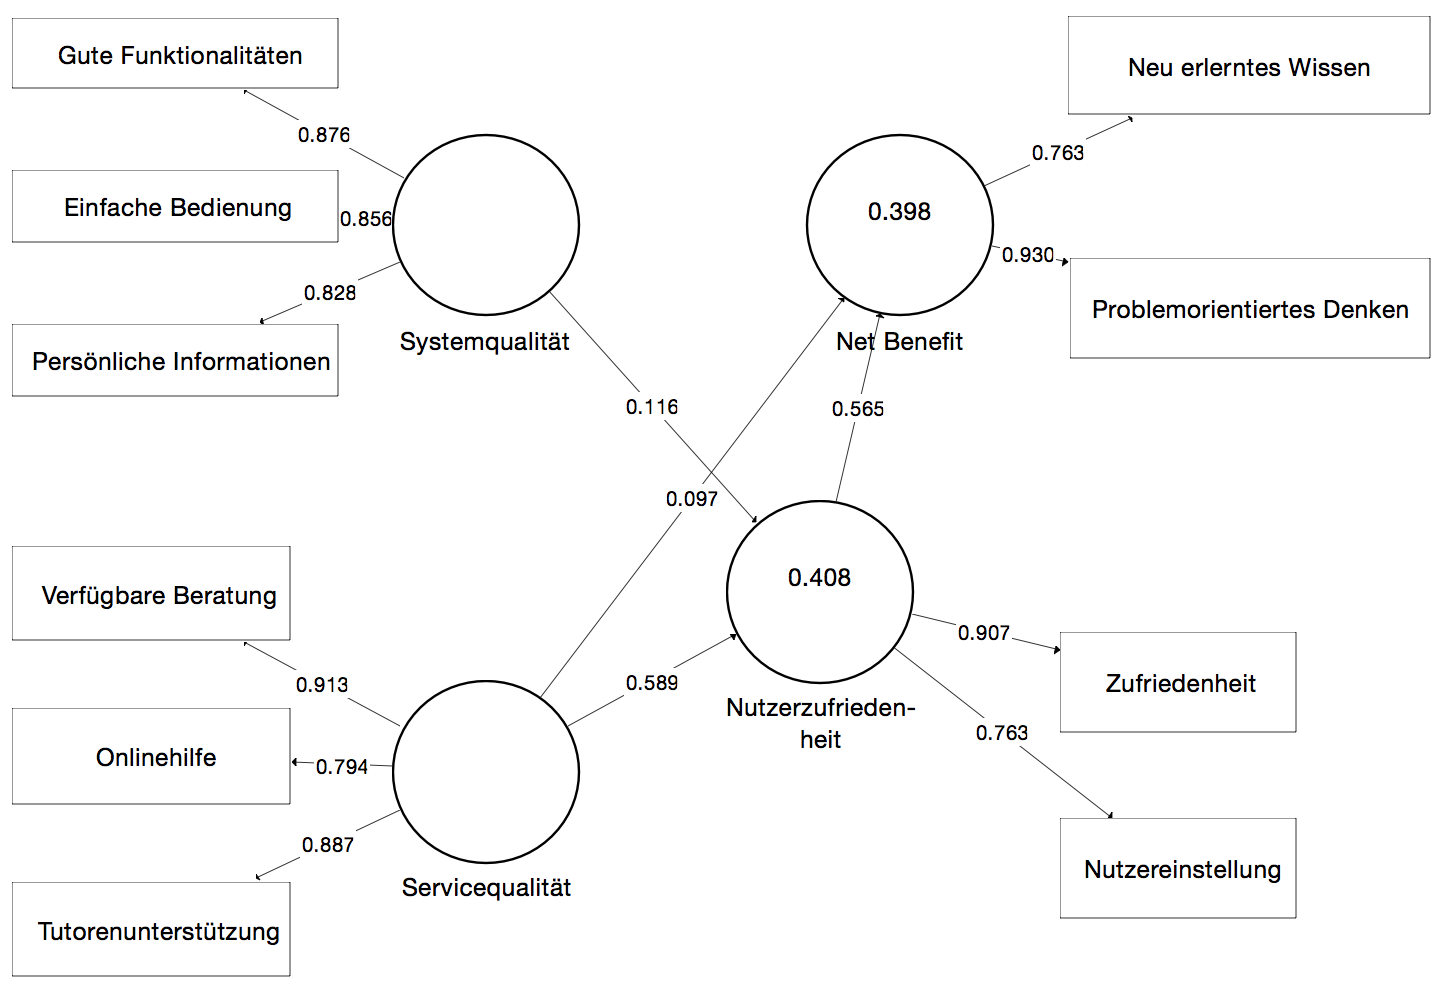
\includegraphics[width=1\textwidth]{Grafiken/pls_bw_3.png}
\caption{PLS Modellergebnisse}
\label{PLS Modellergebnisse}
\end{figure}
\listoffigures 
\listoftables
\printbibliography
\end{document}